\chapter{Baza danych}

\section{Wstęp}
Aby móc wizualizować przebieg pracy systemu wszystkie najważniejsze dane z punktu widzenia automatyki są logowane w bazie danych. Do tego celu wykorzystano bazę danych typu \textit{MYSQL} i środowisko \textit{MYSQL Workbench}, zainstalowane na jednym z komputerów, którym stworzono całą strukturę przedstawioną na rysunku \ref{fig:db}. Dostęp poszczególnych węzłów systemu do bazy danych zapewniony jest poprzez połączenie wszystkich komputerów w lokalną sieci. 
 

\section{Struktura bazy}

Zaprezentowana na rysunku baza danych na strukturę relacyjną aby zapewnić możliwość ewentualnej rozbudowy sytemu o inne składowe. Z racji na to, że baza służy głównie do logowania pracy systemu podzielono ją na następujące części:
\begin{enumerate}
	\item główną tabele \textbf{history}, w której logowane są wszystkie zdarzenia w kolejności chronologicznej,
	\item tabelę  \textbf{Andon}, w której zapisywane są wszystkie sytuacje alarmowe,
	\item tabelę \textbf{Work}, do której logowany jest stan normalnej pracy systemu,
	\item tabelę \textbf{change\_parameter}, w której zapisywane są wszelkie zmiany wartości parametrów systemu,
	\item tabelę \textbf{controller}, która służy do logowania pracy regulatorów.
\end{enumerate}
%
Dodatkowo:
\begin{enumerate}
	\item w tabeli \textbf{state\_space} zdefiniowano wszystkie zmienne stanu występujące w systemie,
	\item tabele \textbf{variable\_state} definiuje wszystkie możliwe stany danej zmiennej np. Work, Andon, Change parameter itd.
	\item tabela \textbf{limits} definiuje poszczególne limity i przypisuje je do odpowiednich zmiennych stanu z tabeli \textbf{state\_space},
	\item w tabeli \textbf{system\_parameter} zdefiniowane są pozostałe parametry systemu takie jak: nastawy poszczególnych regulatorów, wartości zadane itp.
\end{enumerate}

\newpage
\begin{figure}[H]
	\centering
	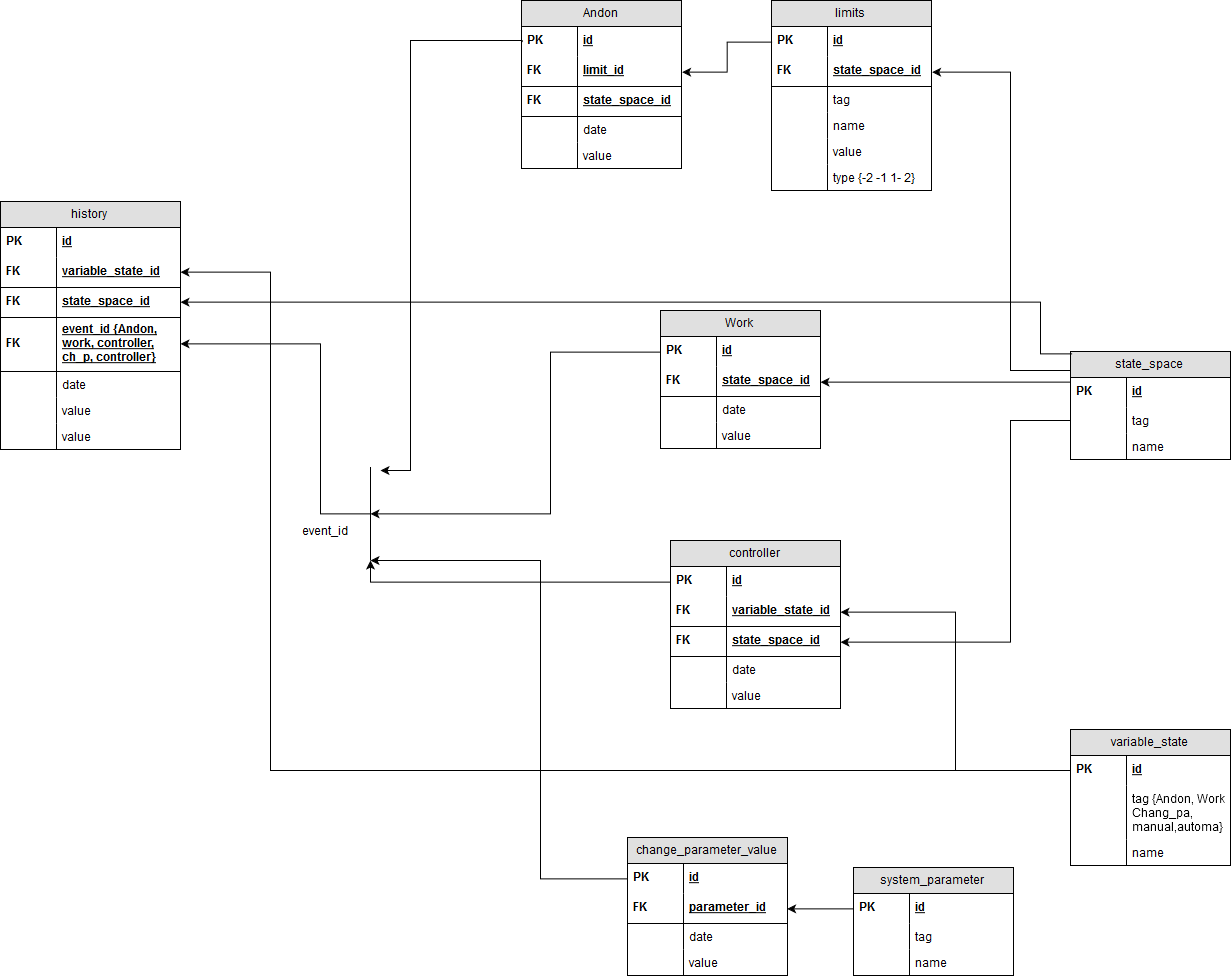
\includegraphics[scale = 0.4]{fig/DB_SCHEMA.png}
	\caption{Struktura bazy danych.}
	\label{fig:db}
\end{figure}

\section{Opis dostępu do bazy}

Dane dotyczące parametrów systemu w poszczególnych chwilach czasu są logowane przez serwer OPC i następnie prezentowane w aplikacji.  